%% This is an example first chapter.  You should put chapter/appendix that you
%% write into a separate file, and add a line \include{yourfilename} to
%% main.tex, where `yourfilename.tex' is the name of the chapter/appendix file.
%% You can process specific files by typing their names in at the 
%% \files=
%% prompt when you run the file main.tex through LaTeX.
\chapter{State of the Art}
The problem of human action classification or pedestrian intent prediction from a sequence of images has got huge attention from the researchers in recent years. This problem is inherently complex as it is based on other 
complex problems. To detect the action or intention one must first detect the object in an image and classify it. Track the same object over several continuous frames to identify the intention. There are several proposals proposed for person detection, many of them try to achieve high accuracy at the expense of high computational cost. This leads many of such proposal not useful for real time application such driver-less cars.   
Before the dominance of convolutional neural network (CNN) and Deep Learning which has outperformed other traditional methods in the recent times. Several researchers found some interesting and great methods, some such nice work done by researchers in these area shall be presented and discussed in the subsequent sections. In general we can think of two types activity prediction, (i) early activity detection (ii) future activity prediction. In the case of early activity detection, the class label of an action is inferred at the point when the activity starts or shortly after the activity started. Where as in the future activity prediction, the class label of the action that will happen next is predicted and also the starting time in the future is also predicted. For any of such prediction task we need efficient and robust object detection, object localization and object tracking model working seamlessly together to enable last phase of the Intent prediction task. Object detection and localization constitute the back bone of this pipe line and takes maximum share of the run time in the entire pipeline. To build a real time pedestrian intention prediction pipeline, it is utmost important to find a model that performs real time object detection and localization reliably. In this chapter some of the state-of-the-art models for such tasks is explored.

\section{Object detection}
Object detection is the core for pose estimation and object tracking. The accuracy of this stage very important for other stages to perform. This detection stage identify the object and locates it. In this section various new algorithms are discussed those deals with object detection.
\subsection{DPM model based on manual feature extraction}
Pedro F. Felzenszwalb and team proposed deformable part model (DPM) \cite{felzenszwalb2009object} which is based on pictorial structures that represent objects by means of a collection of object parts arranged in a deformable configuration. Each object part captures local appearance properties of
an object and the deformable configuration is identified by spring-like connections between certain pairs of such parts. They use a variation of Support Vector Machine(SVM) which they named as latent SVM (LSVM) is used for the training of the model and  histogram of oriented gradients (HOG) used for features vector. After the success of usages of CNNs in tasks like image classification, CNNs are used to extract the feature sets instead of manual extraction.

\subsection{HOG }
In year 2005 Dalal \& Triggs found a method which is superior to Haar wavelets descriptor and other state-of-the-art method based on edge and gradient, at that time for the task of pedestrian detection. HOG descriptors are comparable with edge orientation histogram, SIFT \footnote{Scale Invariant Feature Transform, by transforming image data into scale invariant co-ordinates relative to local features \cite{lowe2004distinctive}} descriptors and shape context, however these are computed on a dense grid of uniformly spaced cell and use overlapping local contrast normalization. Which they named as Histograms of Oriented Gradient (HOG) features\cite{dalal2005histograms}. The gradient is computed by applying a filter kernel \\
\begin{center}
$[-1,0,1] \, and \, [-1,0,1] ^{T}$
\end{center}

\newpara After computation of the gradient they are gradient values are used to update a 9 histogram channel which are evenly spread over 0-180 degrees or 0-360 degrees. They tried peson/non-person classification using this robust feature descriptor and Linear SVM and got state-of-the-art result of that time.

\subsection{CNN based feature extraction}
\newpara CNNs found to be outperform manual feature extraction as they are principally designed Neural net \textbf{architecture which preserves local connections and shares weights}. CNN are special type of multilayer perceptrons, based shared weight architecture and inspired by biological connectivity between neurons in human visual cortex. A particular neuron respond to stimuli only in a restricted region of the visual field called receptive field. CNNs employs a special kind of linear operation called convolution. CNN is characterized by series of several convolution, non-linearity, pooling operation and finally followed by one or more fully connected layers. Initial convolutional layers are used as feature extraction and final layers as fully connected. Fully connected layer takes the input from convolutional network and produces a an N-dimensional vector, where N is the number of classes model is intended to select.

\begin{figure}[h]
	\centering
	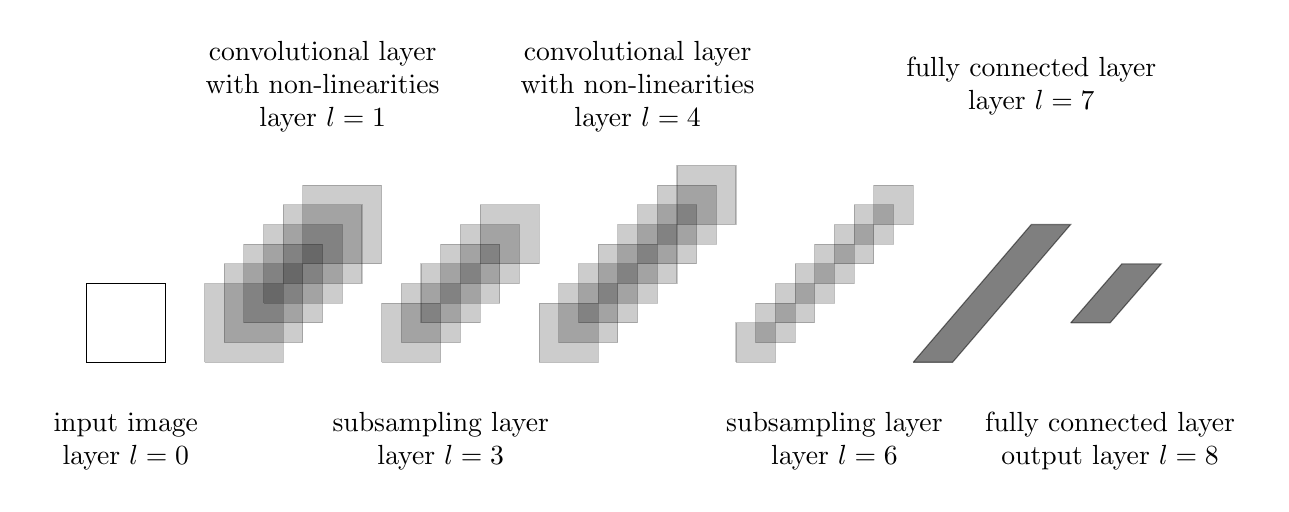
\begin{tikzpicture}
		\node at (0.5,-1){\begin{tabular}{c}input image\\layer $l = 0$\end{tabular}};
		
		\draw (0,0) -- (1,0) -- (1,1) -- (0,1) -- (0,0);
		
		\node at (3,3.5){\begin{tabular}{c}convolutional layer\\with non-linearities\\layer $l = 1$\end{tabular}};
		
		\draw[fill=black,opacity=0.2,draw=black] (2.75,1.25) -- (3.75,1.25) -- (3.75,2.25) -- (2.75,2.25) -- (2.75,1.25);
		\draw[fill=black,opacity=0.2,draw=black] (2.5,1) -- (3.5,1) -- (3.5,2) -- (2.5,2) -- (2.5,1);
		\draw[fill=black,opacity=0.2,draw=black] (2.25,0.75) -- (3.25,0.75) -- (3.25,1.75) -- (2.25,1.75) -- (2.25,0.75);
		\draw[fill=black,opacity=0.2,draw=black] (2,0.5) -- (3,0.5) -- (3,1.5) -- (2,1.5) -- (2,0.5);
		\draw[fill=black,opacity=0.2,draw=black] (1.75,0.25) -- (2.75,0.25) -- (2.75,1.25) -- (1.75,1.25) -- (1.75,0.25);
		\draw[fill=black,opacity=0.2,draw=black] (1.5,0) -- (2.5,0) -- (2.5,1) -- (1.5,1) -- (1.5,0);
		
		\node at (4.5,-1){\begin{tabular}{c}subsampling layer\\layer $l = 3$\end{tabular}};
		
		\draw[fill=black,opacity=0.2,draw=black] (5,1.25) -- (5.75,1.25) -- (5.75,2) -- (5,2) -- (5,1.25);
		\draw[fill=black,opacity=0.2,draw=black] (4.75,1) -- (5.5,1) -- (5.5,1.75) -- (4.75,1.75) -- (4.75,1);
		\draw[fill=black,opacity=0.2,draw=black] (4.5,0.75) -- (5.25,0.75) -- (5.25,1.5) -- (4.5,1.5) -- (4.5,0.75);
		\draw[fill=black,opacity=0.2,draw=black] (4.25,0.5) -- (5,0.5) -- (5,1.25) -- (4.25,1.25) -- (4.25,0.5);
		\draw[fill=black,opacity=0.2,draw=black] (4,0.25) -- (4.75,0.25) -- (4.75,1) -- (4,1) -- (4,0.25);
		\draw[fill=black,opacity=0.2,draw=black] (3.75,0) -- (4.5,0) -- (4.5,0.75) -- (3.75,0.75) -- (3.75,0);
		
		\node at (7,3.5){\begin{tabular}{c}convolutional layer\\with non-linearities\\layer $l = 4$\end{tabular}};
		
		\draw[fill=black,opacity=0.2,draw=black] (7.5,1.75) -- (8.25,1.75) -- (8.25,2.5) -- (7.5,2.5) -- (7.5,1.75);
		\draw[fill=black,opacity=0.2,draw=black] (7.25,1.5) -- (8,1.5) -- (8,2.25) -- (7.25,2.25) -- (7.25,1.5);
		\draw[fill=black,opacity=0.2,draw=black] (7,1.25) -- (7.75,1.25) -- (7.75,2) -- (7,2) -- (7,1.25);
		\draw[fill=black,opacity=0.2,draw=black] (6.75,1) -- (7.5,1) -- (7.5,1.75) -- (6.75,1.75) -- (6.75,1);
		\draw[fill=black,opacity=0.2,draw=black] (6.5,0.75) -- (7.25,0.75) -- (7.25,1.5) -- (6.5,1.5) -- (6.5,0.75);
		\draw[fill=black,opacity=0.2,draw=black] (6.25,0.5) -- (7,0.5) -- (7,1.25) -- (6.25,1.25) -- (6.25,0.5);
		\draw[fill=black,opacity=0.2,draw=black] (6,0.25) -- (6.75,0.25) -- (6.75,1) -- (6,1) -- (6,0.25);
		\draw[fill=black,opacity=0.2,draw=black] (5.75,0) -- (6.5,0) -- (6.5,0.75) -- (5.75,0.75) -- (5.75,0);
		
		\node at (9.5,-1){\begin{tabular}{c}subsampling layer\\layer $l = 6$\end{tabular}};
		
		\draw[fill=black,opacity=0.2,draw=black] (10,1.75) -- (10.5,1.75) -- (10.5,2.25) -- (10,2.25) -- (10,1.75);
		\draw[fill=black,opacity=0.2,draw=black] (9.75,1.5) -- (10.25,1.5) -- (10.25,2) -- (9.75,2) -- (9.75,1.5);
		\draw[fill=black,opacity=0.2,draw=black] (9.5,1.25) -- (10,1.25) -- (10,1.75) -- (9.5,1.75) -- (9.5,1.25);
		\draw[fill=black,opacity=0.2,draw=black] (9.25,1) -- (9.75,1) -- (9.75,1.5) -- (9.25,1.5) -- (9.25,1);
		\draw[fill=black,opacity=0.2,draw=black] (9,0.75) -- (9.5,0.75) -- (9.5,1.25) -- (9,1.25) -- (9,0.75);
		\draw[fill=black,opacity=0.2,draw=black] (8.75,0.5) -- (9.25,0.5) -- (9.25,1) -- (8.75,1) -- (8.75,0.5);
		\draw[fill=black,opacity=0.2,draw=black] (8.5,0.25) -- (9,0.25) -- (9,0.75) -- (8.5,0.75) -- (8.5,0.25);
		\draw[fill=black,opacity=0.2,draw=black] (8.25,0) -- (8.75,0) -- (8.75,0.5) -- (8.25,0.5) -- (8.25,0);
		
		\node at (12,3.5){\begin{tabular}{c}fully connected layer\\layer $l = 7$\end{tabular}};
		
		\draw[fill=black,draw=black,opacity=0.5] (10.5,0) -- (11,0) -- (12.5,1.75) -- (12,1.75) -- (10.5,0);
		
		\node at (13,-1){\begin{tabular}{c}fully connected layer\\output layer $l = 8$\end{tabular}};
		
		\draw[fill=black,draw=black,opacity=0.5] (12.5,0.5) -- (13,0.5) -- (13.65,1.25) -- (13.15,1.25) -- (12.5,0.5);
	\end{tikzpicture}
	\caption[Architecture of a traditional convolutional neural network.]{\protect\cite{davidstutz2016} The architecture of the original convolutional neural network, as introduced by LeCun et al. (1989), alternates between convolutional layers including hyperbolic tangent non-linearities and subsampling layers. In this illustration, the convolutional layers already include non-linearities and, thus, a convolutional layer actually represents two layers. The feature maps of the final subsampling layer are then fed into the actual classifier consisting of an arbitrary number of fully connected layers. The output layer usually uses softmax activation functions.}
	\label{fig:traditional-convolutional-network}
\end{figure}

\newpara \textbf{Convolution layer} It is the first layer to which, the input image is given. A small matrix otherwise known as a filter or kernel moves along the image and is convoluted with the input image. As a process of convolution \ref{fig:Schematic-representation} kernel elements are multiplied with the original pixel value and these values are summed up and produces a feature map as input for further layers.
 
\newpara \textbf{Nonlinear layer}
A non-linearity is added to the output generated from a convolution layer in the form of an activation function in this layer. The basic idea of adding a non-linear layer is to make different layers within the network have a non-linear relationship and this ensures the network can make more complex decisions.
Usually ReLU is used as a non-linear activation function and mathematically given as below.
%https://machinelearningmastery.com/rectified-linear-activation-function-for-deep-learning-neural-networks/

\begin{equation}
	f(x) =max(0, x)
\end {equation}
Where x is the input to a neuron and output is similar to ramp function.
Although simple, it has been demonstrated that this activation function enables better performance in deeper networks compared to widely used complex function such as \textit{sigmoid} (fig:\ref{fig:Sigmoid-function}) and \textit{hyperbolic tangent} (fig: \ref{fig:tanh-function}).

\newpara \textbf{Pooling layer}
The subsequent layer after non-linear layer. It down samples the the image, as a result the processed image volume is reduced. Max-pooling is similar to convolution, but it chooses the maximum element within the area where the maxpool filter is applied. For a pooling size (2,2) the input is halved in both spatial dimensions.

\newpara \textbf{Fully connected layer}
Normally a fully connected layer is attached to the Network as last layer of the Network. Fully connected layer performs classification by taking input as features extracted and transformed in the previous conv-relu-pooing layers. This results in an N dimensional vector, where N is the number of classes the model is trained on.

\newpara CNN learns the filters that traditional image classification algorithm hand crafts. This makes CNN little pre-processing compared to other traditional algorithm and results superior results. There are many evolution of CNNs starting from LeNet (LeCun et al., 1989) for zip code recognition, LeNet-5 (1998) a 7 layer CNN \ref{fig:traditional-convolutional-network} by LeCun et al. for hand written numbers on the check recognition, AlexNet by Alex Krizhevsky et al. in 2012 used deeper layers and more filters per layer than leNet-5. It also used ReLU activation, max pooling, dropout, data agumentation and SGD with momentum during training. \footnote{These terms shall be discussed in the subsequent chapter.} This achieved a record breaking result at that time. ZFNet in 2013 winner of ILSVRC 2013 with a small tweaking to AlexNet. 2014, GoogleNet otherwise known as Inception V1 from Google achieved human level performance. Another net in the same year got the attention known as VGGNet. It uses only 3x3 convolution, 16 layers and with lots of filters. It consists of 138 million parameters and one of major disadvantage and required more time to train. And weight configuration of this is publicly available and used as baseline feature extractor.

\section {Object Localization } Object localization is one step forward when compared to object recognition. Identifying whether an object is present in the image or not is the task of object recognition, however object localization deals with locating where the object is located in an image. There are several approaches used for localization as discussed below. And it is complex in comparison to image classification because huge number of candidate object locations must be processed during the localization process. \\

\textbf{Sliding Window:} A classifier is trained on the objects first and in the next phase a window is moved over whole image at different scales. Each window gets a score from the learned classifier and window(s) with the highest score predicts the location of an object. Sliding Window technique is computationally inefficient. Some of the improved and modern methods are presented below. 

\subsection{R-CNN Introduction}
In \cite{girshick2014rich} Girshick et al. combined region proposals with CNN and naming the method as R-CNN. This method generates around 2000 category independent region proposals for the input image, using a CNN, a fixed length feature vector is extracted regardless of the region shape. Then each region is classified using class specific linear SVM. 

\newpara \textbf{R-CNN:} \\
The features for a region proposal is computed via a CNN proposed by Krizhevsky et al. This network takes mean-subtracted 227 x 227 RGB image as input. Therefore image data in the region proposal is converted to 227 x 227 as required by Krizhevsky network. For this arbitrary-shaped  proposed region is dilated and warped. During the test time using selective search fast mode 2000 region proposals are generated and warped and processed through CNN to extract desired features. After that per class basis score is evaluated using the SVM trained for that class. Subsequently a greedy non-max suppression for each class independently is applied which rejects region that has IoU overlap with higher scoring selected region larger than a threshold.

\newpara \textbf{Fast R-CNN:} \\
In \cite{girshick2015fast} an improved technique is discussed which is based on previously discussed R-CNN. This is computationally faster than R-CNN ans results in faster training and testing speed. R-CNN training was a multi-stage pipeline. It first fine tunes a ConvNet on object proposal and then fits SVMs to ConvNet features. Because of feature extraction from each object proposal, without sharing computation in each test image, object detection was relatively slow in R-CNN. Based on the concept described in SPPnets, a convolutional feature map is generated for entire input image and subsequent classification is done by extracting features from the shared feature map for each object proposal. Features for the object proposal is extracted by max-pooling the portion of feature map inside the  object proposal region into a fixed size output. During the training, Fast R-CNN takes an entire image and set of object proposals, for each object proposal an RoI layer extract a fixed length feature vector from the feature map. Each feature vector is further fed into fully connected layers which produces a feature vector that is branched into two output layers, one outputs softmax probability over K object classes and other layer produces four real numbers for each of the K object classes termed as bbox regressor. The architecture is trained with multi-task loss function via back propagation. Fast R-CNN uses softmax classifier instead of linear SVM that was used in R-CNN.

\newpara \textbf{Faster R-CNN:} \\  
Another enhanced proposal came from Author of previously discussed R-CNN methods with a goal of sharing computation with a Fast R-CNN for the task of region proposal. In \cite{ren2015faster}, a new Region Proposal Network (RPN) is introduced that shares full image convolutional features with the detection network, thus almost eliminating the cost for the region proposals. RPN is a fully convolutional network that simultaneously predicts object bounds and objectness scores at each position. This RPN is trained to generate high quality region proposals, which are used by Fast R-CNN for detection. By sharing convolutional layers with the object detection network, RPN has marginal cost for computing proposal is small \footnote{in the order of 10 ms per image}. For the very deep VGG-16 model this methodology achieved 5fps on GPU and accuracy of 73.2\%mAP for PASCAL VOC 2007 using 300 proposals per image. 

\subsection{Model based on R-CNN}
\newpara Estimating pedestrian future using pedestrian dynamic model were done in the past and these models are difficult to adjust and to achieve robustness, they require high quality stereo data, dense optical flow and ego-motion compensation which requires vehicle data.  Using the 2D pose estimation method, that is applied to the still images in sliding window manner, a state of-the-art result has been obtained\cite{fang2018pedestrian} for the C/NC task with Daimler dataset. In the pipeline of their task they used below components. They have used generic off-the-shelf CNN modules as Detector, Tracker and Pose Estimator in their pipeline.

\begin{itemize}
	\item Detection: Fine tuned Faster R-CNN \cite{ren2015faster} based on VGG16 CNN architecture. 
	\item Tracking: Object tracking-by-detection \cite{wojke2017simple}, purely image based of-the-shelf solution 
	\item Pose Estimation: CNN-based pose estimation method discussed in \cite{cao2017realtime}
	\item Prediction: Random Forest based on 4096T dimensional vector, where T is number of frames tracked
\end{itemize}

\newpara
Researcher Fang and team in their 2018 paper \cite{fang2018pedestrian} described about image based 2D pose estimation for detecting pedestrian intention: whether the pedestrian crossing the road, stopping before entering the road, starting to walk or bending towards the road. They performed their experiment with choreographed Daimler dataset. They also used publicly available, a rather new dataset (JAAD) \cite{kotseruba2016joint} that allows development of methods and experiment in a more naturalistic driving condition. They used CNN based pedestrian detection, tracking and pose estimation to predict the crossing action from monocular images. In their paper they have mentioned that without additional information such as stereo, optical-flow or ego-motion compensation, they achieved the state-of-the-art results with only image-based 2D pose estimation. The prediction of the action is based on per pedestrian multi-frame feature set extracted using last \textit{k} frames. Estimating the pose was central to the prediction of the crossing intention. In the results they have observed that classification with respect to features based on  skeleton of the pedestrian outperform the features based on CNN fc6 layer.

\subsection{Single Shot Multi Box}
SSD motivated by the ideas presented in \cite{szegedy2014scalable} where a convolutional network is trained to output the coordinates of the object bounding boxes. MultiBox loss is the weighted sum of \textit{confidence} loss and \textit{location} loss. Single Shot Multi Box with aforementioned inspiration attacked the problem with several small improvements and variation achieving state-of-the art results with still simpler architecture, in comparison to \cite{szegedy2014scalable} which uses a separate deep neural network to generate proposal for the bounding box.
\subsubsection{SSD}
Faster R-CNN, operates at only 7 frames per second (FPS) SSD aimed at improving the speed by employing some new methods which does not re-samples pixels or features for the bounding hypothesized boxes. This improves the speed substantially with out much or no decrease in accuracy. 

\newpara The central principle on which SSD \cite{liu2016ssd} is based on is, discretizing the output space of bounding boxes into a set of pre-determined default boxes consisting of different aspect ratios and scale per feature map location. The principle used as part of SSD overcomes the challenge faced in \cite{ren2015faster} and its predecessors which includes multi phase training and slow inference time. SSD does this by doing both the task of object localization and classification in a single forward pass. It uses a \textit{MultiBox} approach, which pre-computes priors \footnote{Alternatively known as anchors in Faster R-CNN}, fixed size bounding boxes. In MultiBox based approach, prediction starts with priors and try to regress closer to the ground truth bounding boxes.
It uses combination of confidence loss and location loss for calculating the loss of the model. Confidence loss uses categorical cross-entropy \footnote{otherwise known as softmax loss} and location loss uses Smooth L1-Norm \footnote{\textit{L1}-norm is well known as \textit{Manhattan }norm}.

\begin{equation}
	\left \| x_1 \right \| =\sum_i(x_{1_i})
\end {equation}

L1-norm gives distance between two vectors, known as \textit{Sum of Absolute Difference} distance given by below equation:
\begin{equation}
	SAD(x_1,x_2) = \left \| x_1-x_2 \right \|_1 = \sum \left | x_{1_i}-x_{2_i} \right |
\end {equation}

\textbf{Fixed Priors:} In case of MultiBox, the priors are chosen according to their IoU with respect to ground truth above a certain defined ratio. \footnote{Usually 0.5 is considered as threshold value}.
However, in case of Fixed Priors, carefully, a set of different size and aspect ratio priors are chosen manually. This lead to removal of pre-training phase for the prior generation. For a feature map with \textit{b} default bounding boxes per cell and model is trained for \textit{c} classes, then the number of values for the feature map is given by the relation 
\begin{equation}
	f = (m * n )  (4 + c) * b
\end {equation}
4 in the above equation indicates number of co-ordinate values for two corner points or 4 offset relative to the original default box shape. \\
m x n is the shape of the feature map \\
 Additional point to note is, more the number of default boxes, the more accurate is the detection at the cost of speed.
Predicting category scores for multiple classes and box offsets for pre-computed bounding boxes using a small convolutional filters applied to feature maps lead to a faster single pass object classification and localization system. And prediction of different scales from feature maps of different scales and separate prediction by aspect ratio leads to higher accuracy. \cite{liu2016ssd} With same VGG-16 base architecture SSD300 model runs at 59 FPS. The mentioned result from SSD paper is very interesting and suitable for application of recurrent neural network to detect and track object in video simultaneously in real time.

\subsubsection{YOLO}
Another variation of single shot detection during the same time achieving the state-of-the-art result was YOLO. Single network based detection pipeline. YOLO divides the image into a grid of cells and predicts the coordinates and confidences of objects contained in the cells. Authors like Szegedy et.al in \cite{szegedy2014scalable} has expressed uncertainty about its performance in the situation where there are significantly more objects in a data set. As SSD seems to performs better with respect to run time and performance, YOLO was not studied further during Thesis period.

\subsection{Network architectures}

Standard CNN architectures, over the last 2 decades uses set of standard layer that can be graphically \ref{tomepel} represented as below. 

\begin{figure}[h]
\begin{align*}
\begin{tikzpicture}[baseline=-3pt]
\node[] at (0,0) {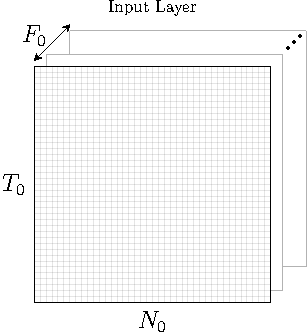
\includegraphics[scale=0.5]{input_layer}};
\end{tikzpicture}&=
%
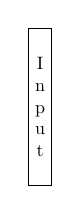
\begin{tikzpicture}[baseline=-0pt]
\draw (0,-1) rectangle (0+0.3,1);
\node[align=center,scale = 0.65] at (0+0.15,0) {I \\ n \\ p \\ u \\ t};
\end{tikzpicture}\;,&
%
\begin{tikzpicture}[baseline=-3pt]
\node[] at (0,0) {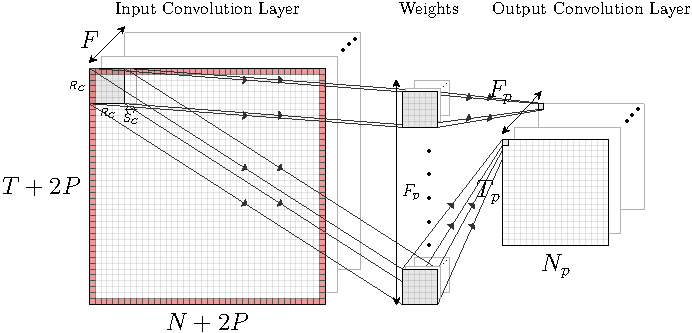
\includegraphics[scale=0.5]{VGG-conv}};
\end{tikzpicture}&=
%
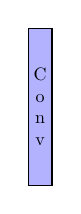
\begin{tikzpicture}[baseline=-0pt]
\filldraw[fill=blue!30!white] (0,-1) rectangle (0+0.3,1);
\node[align=center,scale = 0.65] at (0+0.15,0) {C \\ o \\ n \\ v};
\end{tikzpicture}\;,\notag\\
%
\begin{tikzpicture}[baseline=-3pt]
\node[] at (0,0) {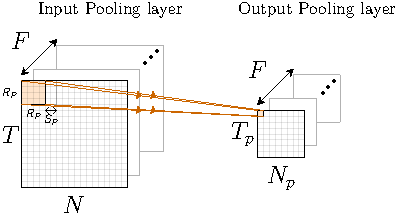
\includegraphics[scale=0.5]{VGG-pool}};
\end{tikzpicture}&=
%
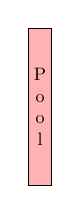
\begin{tikzpicture}[baseline=-0pt]
\filldraw[fill=red!30!white] (0,-1) rectangle (0+0.3,1);
\node[align=center,scale = 0.65] at (0+0.15,0) {P \\ o \\ o \\ l};
\end{tikzpicture}\;,&
%
\begin{tikzpicture}[baseline=-3pt]
\node[] at (0,0) {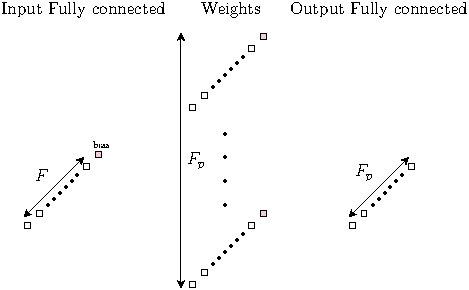
\includegraphics[scale=0.5]{VGG-fc}};
\end{tikzpicture}&=
%
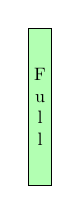
\begin{tikzpicture}[baseline=-0pt]
\filldraw[fill=green!30!white] (0,-1) rectangle (0+0.3,1);
\node[align=center,scale = 0.65] at (0+0.15,0) {F \\ u \\ l \\ l};
\end{tikzpicture}
\end{align*}
\begin{center}
\caption{CNN layers: Schematic representation}
\label{fig:Schematic-representation}
\end{center}
\end{figure}

\newpara Based on these schematic layers, a simple graphical \footnote{\label{tomepel} Images source: Thomas Epelbaum GitHub: https:\textbackslash github.com\textbackslash tomepel\textbackslash Technical\_Book\_DLaccessed on 07th August 2019 } representation of VGG-Net is shown below.
\begin{figure}[h]
\begin{center}
\begin{tikzpicture}
\node[] at (0,0) {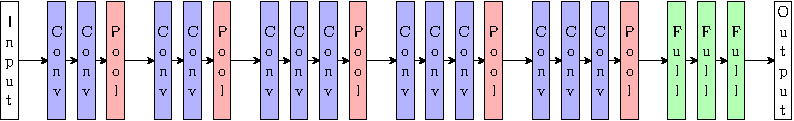
\includegraphics[scale=1]{VGG}};
\end{tikzpicture}
\caption{VGG-Net}
\end{center}
\end{figure} 

\section{Tracking}
Visual object tracking is also a very active area of research, increasing number of algorithms are being proposed.
In \cite{fiaz2019handcrafted} Fiaz et. al broadly categorized trackers into o Correlation Filter based Trackers (CFTs) and Non-CFTs. Human trackers can be divided into motion model or appearance model. They experimented with 24 recent trackers and found that trackers using deep features performed better than handcrafted. In some cases fusion of both increases performances significantly. Based on their study they have concluded that Discriminative Correlation Filter (DCF) based trackers perform better than others. There are some notable implementation e.g. 
Kalman Filter with Mean shift tracking, Recurrent YOLO, a deep neural network that uses raw video frames as input and its output is the coordinates of a bounding box of an object being tracked in each frame.
More in-depth research was out of the scope of the Thesis topic, so no much study was done in this area.

\section{Prediction}
The last stage of the pipeline which actually predicts the future location of the visual object. Predicting  bounding box for a tracked pedestrian. Predicting intention of the pedestrian, whether pedestrian wants to cross in near future or not. Subsequent section shall discuss about some of the state-of-the art methodology that address this.

\subsection{RNN}
Recurrent neural network primarily are densely connected neural network similar to feed forward network with a key difference; introduction of \textit{time} component in RNN. The output of a hidden layer in an RNN is \textit{fed back } into itself. With this we can model the data which is time dependent or sequence dependent in nature. In programming terms this can be represented by a fixed program taking certain inputs and some internal variable.
\begin{center}

\begin{tikzpicture}[item/.style={circle,draw,thick,align=center},
itemc/.style={item,on chain,join}]
 \begin{scope}[start chain=going right,nodes=itemc,every
 join/.style={-latex,very thick},local bounding box=chain]
 \end{scope}
 \node[left=2em,item] (AL) {$A$};
 \path (AL.west) ++ (-1em,2em) coordinate (aux);
 \draw[very thick,-latex,rounded corners] (AL.east) -| ++ (1em,2em) -- (aux) 
 |- (AL.west);
 \draw[very thick,-latex] (AL.north) -- ++ (0,2em)
 node[above,item,fill=gray!10] {$h_t$};
 \draw[very thick,latex-] (AL.south) -- ++ (0,-2em)
 node[below,item,fill=gray!10] {$x_t$};
\end{tikzpicture}

\end{center}

\newpara The above diagram depicts a compact loop form of an RNN showing a loop. An RNN can be thought as a multiple copies of the same network, each previous network passing a message to it successor. By unrolling the compact for we can visualize the RNN as below. 

\begin{center}

\begin{tikzpicture}[item/.style={circle,draw,thick,align=center},
itemc/.style={item,on chain,join}]
 \begin{scope}[start chain=going right,nodes=itemc,every
 join/.style={-latex,very thick},local bounding box=chain]
 \path node (A0) {$A$} node (A1) {$A$} node (A2) {$A$} node[xshift=2em] (At)
 {$A$};
 \end{scope}
 \node[left=1em of chain,scale=2] (eq) {$=$};
 \node[left=2em of eq,item] (AL) {$A$};
 \path (AL.west) ++ (-1em,2em) coordinate (aux);
 \draw[very thick,-latex,rounded corners] (AL.east) -| ++ (1em,2em) -- (aux) 
 |- (AL.west);
 \foreach \X in {0,1,2,t} 
 {\draw[very thick,-latex] (A\X.north) -- ++ (0,2em)
 node[above,item,fill=gray!10] (h\X) {$h_\X$};
 \draw[very thick,latex-] (A\X.south) -- ++ (0,-2em)
 node[below,item,fill=gray!10] (x\X) {$x_\X$};}
 \draw[white,line width=0.8ex] (AL.north) -- ++ (0,1.9em);
 \draw[very thick,-latex] (AL.north) -- ++ (0,2em)
 node[above,item,fill=gray!10] {$h_t$};
 \draw[very thick,latex-] (AL.south) -- ++ (0,-2em)
 node[below,item,fill=gray!10] {$x_t$};
 \path (x2) -- (xt) node[midway,scale=2,font=\bfseries] {\dots};
\end{tikzpicture}
\end{center}

Mathematically RNNs can be represented as below: 

\begin{equation}
	\textbf{h}_t = f_W(\textbf{h}_{t-1} + \textbf{x}_{t}) 
\end{equation}

Where \textbf{\textit{ f}} is some function with parameter \textbf{W}. \\
This same function \textbf{\textit{ f}} and same weight matrix \textbf{W} is used at every step of the computation. \\
\textit{$h_t$} is new state \\
\textit{$h_{t-1}$} is old state \\
\textit{$x_t$} input vector at time step \textit{t}\\

In a more simplified form we can have the above function as:

\begin{equation}\label{hidden_state}
	\textbf{h}_t = \sigma (\textbf{Ux}_t + \textbf{Vh}_{t-1}) 
\end{equation}

Where \textit{U} is the input weight matrix and \textit{V} is the recurrent outputs. Time stamp denoted by \textit{t}. $\sigma$ represent an activation function e.g a \textit{tanh} or \textit{sigmoid}. If we unfold the above equation and go back three time step we have,

\begin{equation}
	\textbf{h}_t = \sigma (\textbf{Ux}_t + \textbf{V}(\sigma(\textbf{Ux}_{t-1} + \textbf{V}(\sigma(\textbf{Ux}_{t-2})))
\end{equation}

And in general, if we unfold in n time slot back,

\begin{equation}
\textbf{h}_t = \sigma (\textbf{Ux}_t + ...( \textbf{V}(\sigma(\textbf{Ux}_{t-n+2} + \textbf{V}(\sigma(\textbf{Ux}_{t-n+1})..)))
\end{equation}

\begin{equation}
	\textbf{y}_t = (\textbf{W}_{hy}  \textbf{h}_{t}) 
\end{equation}

Where \textbf{$y_t$}  represents output at a time stamp \textit{t} \\
\textbf{$h_t$} is the hidden state, computed as in equation \ref{hidden_state}

The problem in general suffered by a plain RNN is over a large period of time the back propagation gradients either exploding or vanishing. During a \textit{vanishing gradient } problem, the gradients of the network output with respect to the early layer of the network becomes extremely small, which indicates a large change in the parameters for the early layers does not have a big effect on network output. Usually this happens when the activation function such as \textit{sigmoid} or \textit{tanh} squash their input into a small output range non-linearly. Considering the activation function sigmoid which is defined as below,

\begin{equation}
	S(x) = \frac{1}{ 1+ e^x}
\end{equation}

Sigmoid is a special case of standard Logistic function defined as 
\begin{equation}
f(x) = \frac{L}{ 1+ e^{-k(x-x_0)}}
\end{equation}
Where \\
L: Curve's maximum value \\
k: Steepness of the curve \\
(x0 - x): value of Sigmoid's midpoint \\

A standard logistic function is called sigmoid when (k=1,x0=0,L=1) and can be viewed as below: \\
\begin{figure}[h]
	\centering
	\begin{tikzpicture}
		\begin{axis}%
			[
			grid=major,     
			xmin=-10,
			xmax=10,
			axis x line=bottom,
			ytick={0,.5,1},
			ymax=1,
			axis y line=middle,
			]
			\addplot%
			[
			blue,%
			mark=none,
			samples=200,
			domain=-6:6,
			]
			(x,{1/(1+exp(-x))});
		\end{axis}
	\end{tikzpicture}
	\caption{Sigmoid function}
	\label{fig:Sigmoid-function}
\end{figure}

Sigmoid function can be re written as  \\
\begin{equation}
	S(x) = (1+e^{-x})^{-1}
\end{equation}
And by taking the derivative \\
\begin{equation}
\frac{d}{dx}S(x) = \frac{d}{dx} (1+e^{-x})^{-1} \\
= \frac{e^{-x}} {(1+e^{-x})^{-2}} 
\end{equation}

Plotting the derivative of the sigmoid activation function as below, we notice that 
\begin{center}

\begin{tikzpicture}
\begin{axis}%
[
grid=major,     
xmin=-10,
xmax=10,
axis x line=bottom,
ytick={0,.5,1},
ymax=1,
axis y line=middle,
]
\addplot%
[
blue,%
mark=none,
samples=100,
domain=-10:10,
]
(x,{exp(-x)/((1+exp(-x)) * (1+exp(-x)))});
\end{axis}
\end{tikzpicture}
\end{center}

\begin{figure}[h]
	\centering
	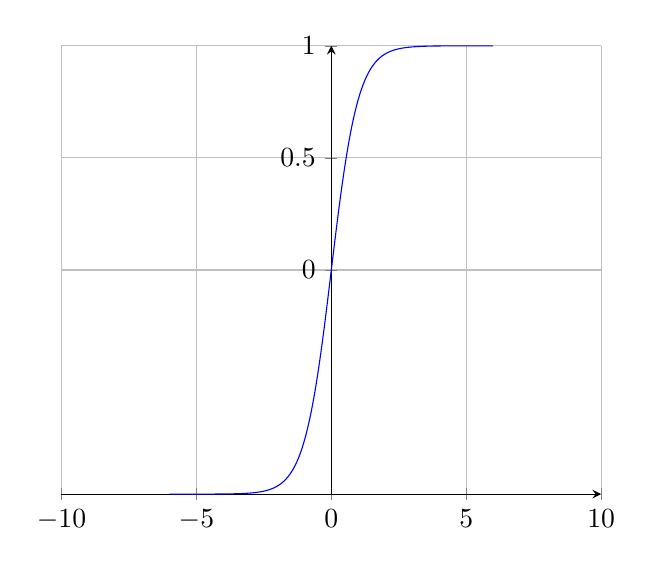
\begin{tikzpicture}
		\begin{axis}%
			[
			grid=major,     
			xmin=-10,
			xmax=10,
			axis x line=bottom,
			ytick={0,.5,1},
			ymax=1,
			axis y line=middle,
			]
			\addplot%
			[
			blue,%
			mark=none,
			samples=200,
			domain=-6:6,
			]
			(x,{(exp(2*x)-1 )/(exp(2*x)+1 )});
		\end{axis}
	\end{tikzpicture}
	\caption{Hyperbolic Tangent Function}
	\label{fig:tanh-function}
\end{figure}


the sigmoid derivative is well below the 1.0 in the whole range of input values. And this makes the gradients vanishing quite fast as, multiplying this value \footnote{value less than 1} several times for several layer \textit{ back propagation} brings the value close to 0.

\subsubsection{Models based RNN }
\newpara Abu Farha and team presented \cite{abu2018will} a similar work, where they discussed methods to predicts action that are considerably in future and their duration. And they tried to anticipate all activities within a horizon of 5 minutes. After inferring the activities from the observed part of the video using an RNN-HMM \cite{richard2017weakly}, they proposed two approaches to predict the future actions and their durations, in the first approach they used RNN, where the anticipated activities are fed to the RNN to predict the remaining duration of the on going activities and duration of the next activity along with its class.
In the second approach the proposed CNN based single pass model which predicts length and label of the future action. They have found that these both approach have outperformed both grammar based baseline and nearest neighbor baseline. RNN and CNN found to be performing similarly for time horizon more than 40 seconds and RNN performs better for lesser than 20 seconds time horizon. The task is more formally defined as,
given the first t frames $X_{\text{1}}^t$ \\
predict \[ C_{t+1}^T  = \ (C_{t+1}, ..., C_{T}) \]
where $C_{\text{i}}$ denotes action labels for unobserved frames
and the video is given by
\[ X_{1}^T = (X_{1}, ..., X_{T}) \]

\newpara
For the RNN training the loss function used as below
\begin{equation}
    L = -log\, \hat{p_c} + (l_r - \hat{l_r})^2 +  I (l_n - \hat{l_n})^2 
\end{equation}
where \\
$\hat{l_r}$ represents predicted remaining length of the current action, \\
$\hat{l_n}$ represents predicted length of the next action, \\
$\hat{p_c}$ is the predicted class of the next action

\newpara Unlike recursive strategy in RNN, CNN approach does the prediction in a one single pass.
Training data generated by using first 10\%, 20\%, 30\%, 50\% of the video as the observation and the following 50\% as the ground truth. During the training of the network squared error used as loss function.
\begin{equation}
    L = \frac{1} {SC} \sum_{a,c} (Y_{sc} - \hat{Y_{sc}})^2 
\end{equation}
where $\hat{Y}$ is the prediction of the network. \\
C represents action classes and \\
S number of rows for an action segment

\newpara Row-wise $\textit{l}_2$-normalization \footnote{$l_2$-norm of a real vector $x=(x_1,x_2,x_3)$ is given by $|x|=sqrt(x_1^2+x_2^2+x_3^2)$} of the output found to be more robust than softmax output with cross-entropy loss. \cite{abu2018will} did not elaborate the 'input sequence always end 1 second before the next action segment start'. What is the purpose of this and results if the input sequence is provided till the next action segment starts.

\subsubsection{Dynamic bag-of-words} 
For the task of early detection, the goal is to recognize the activity with least possible amount of input observation \cite{ryoo2011human}. In \cite{ryoo2011human} they modeled the feature distribution over the course of observation by integral histogram representation of activities, and named the prediction algorithm as \textit{dynamic bag-of-words} as the prediction algorithm considers the sequential structure formed by video features. And they formulated the activity prediction process probabilistically as:
%\hat{f}(x,y) = \underset{(s,t)\in S_{xy}}{\mathrm{median}} \{g(s,t)\}
%\begin{equation}
%\begin{multlined}
\begin{align}
\begin{split}
	%\displaystyle \sum_{n=1}^\infty
		P(A_{p}\: |\: O,t) ={}& \displaystyle \sum_{d}  P(A_{p},d\: |\: O,t)\\
		={}&	\frac{\sum_{d} P(O\: | \: A_{p},d)P(t\: | \:d)P(A_{p},\: d)}
	 {\sum_{i}\sum_{d} P(O\: | \: A_{i},d)P(t\: | \:d)P(A_{i},\: d) }
\end{split}
\end{align}
%\end{multlined}
%\end{equation}

\newpara Where \textit{d} is a progress level of the activity \\
\textit{$A_{p}$}  \textit{ P(t|d)} represents the similarity between the observation length \textit{t} and that of the activity progress \textit{d}
\textit{P(O|Ap, d)} measures the similarity between the video observation and the activity \textit{$A_{p}$} with progress level \textit{d}. This \textit{integral bag-of-words} uses 3-D space-time local features and detect motion changes in the video and generates descriptors representing local movements in the video. These are cuboid feature descriptors \cite{dollar2005behavior}. After the features are extracted, \textit{k-means} clustering was applied and the clusters are knows as visual words. Every feature detected is now belong to one of this k-visual words. Then the activities are model as an integral histogram of visual-words. The similarity between a video and activity model was done by comparing their histogram representation. And finally dynamic programming was used to predict the ongoing activities from videos.

\subsection{LSTM}
LSTM has a chain like structure as in RNN but the repeating module has a different structure. There are four neural network layer as contrast with RNN that has a single neural network layer. The four neural network layers interact in a very special way. LSTM networks have gained acceptance for time sequence data processing, such as image captioning, action recognition, speech recognition, language translation etc. An LSTM visually can be shown as below. 

\begin{figure}[h]
\begin{align*}
\begin{tikzpicture}[baseline=-3pt]
\node[] at (0,0) {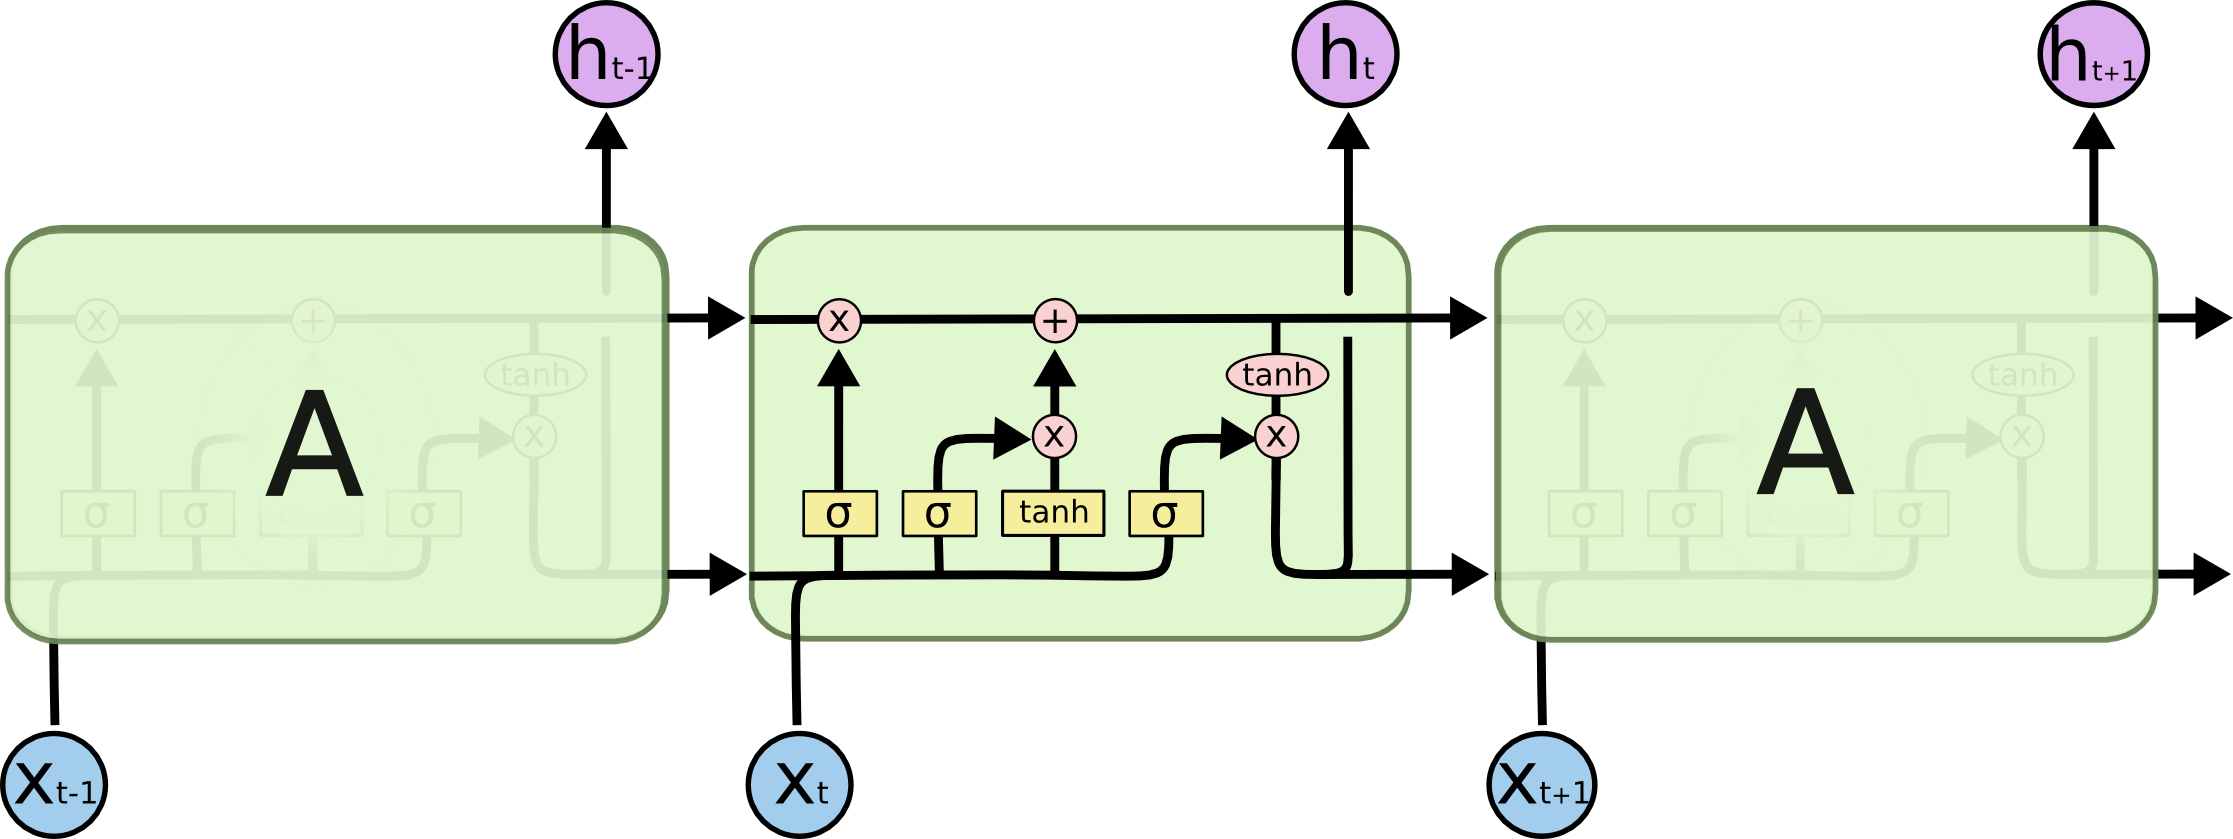
\includegraphics[scale=0.5]{LSTM3-chain}};
\end{tikzpicture}&
\end{align*}
\begin{center}
\caption{LSTM schematic diagram, diagram source:\cite{christopherolah}}
\end{center}
\end{figure} 

The core idea to LSTM is the cell state, it run through the entire chain and performs some minor linear interaction. LSTM adds or removes information to the cell state with the help of regulated structure called gates. Gates are represented by a neural network layer sigmoid activation and a point-wise multiplication operation.
A sigmoid outputs how much of a component should be let through. A value of 0 blocks the whole component and a value of 1 let entire component through. In a basic LSTM, there are four such gates.
With arrival of new information, the model first decides which long term information is not needed anymore, and forgets it. Stores necessary part of the new information into long-term memory. An LSTM has three such gates, that controls the cell state.
A \textbf{remember gate} is learned that takes new input and working memory as input and outputs \textit{n} bummers between 0 and 1, each determines degree to which long-term memory element to be kept. Where 1 indicates to keep it and 0 indicates to forget it entirely. A small neural network can model this \textbf{remember gate} given below. In the literature this is also known as \textbf{forget gate}.

\begin{equation}
f_t = \sigma(W_f. [h_{t-1}, x_t  ] + b_f)
\end{equation}
Where $W_f$ is the weight matrix for the forget gate \\
$h_{t-1}$ is the cell state at time (t-1) \\
$b_f$ is the bias for the forget gate

After forgetting the unnecessary information, LSTM is interested in storing the new required information in the cell state. This involves two step, with a \textbf{input} sigmoid layer values that needs to be updated is decided. And then a tanh layer creates a vector for new candidate values for cell state that could be added to the cell state. 

\begin{equation}
i_t = \sigma(W_i. [h_{t-1}, x_t  ] + b_i)
\end{equation}

\begin{equation}
C_t\textasciitilde = tanh(W_C. [h_{t-1}, x_t ] + b_C)
\end{equation}

Both $i_t$ and $C_t\textasciitilde$ is combined to update the cell state as below.

\begin{equation}
C_t = f_t * C_{t-1} + i_t * C_t\textasciitilde
\end{equation}

Next, output is decided based on cell state and a output gate, that decides what part of the cell state are going to output. Mathematically this can be represented as below.

\begin{equation}
o_t = \sigma(W_o. [h_{t-1}, x_t  ] + b_o)
\end{equation}
\begin{equation}
h_t = o_t  * tanh(C_t)
\end{equation}

There are several variants of LSTM, but basic variant was explored and used in the scope of the Thesis.

\subsection{Models based on LSTM }
In \cite{saleh2017intent} Saleh et.al presented a data driven approach which is different from older approach which employs dynamical motion modelling and motion planning. They have formulated the the intent prediction problem as a time-series problem. They proposed the method by observing a short window sequence of the pedestrian motion trajectory, a prediction about their future latent position can be done up to 4 secs ahead. With a deep stacked LSTM network they achieved competent results on Diamler testing data set. In their work, three LSTM layers are stacked. The input layer takes 2-dimension sequence with a window size 10 of lateral position of pedestrian motion trajectory. Last LSTM layer connected to a fully connected layer which has only one neuron and predicts lateral position at the next time step. A linear activation function is used in the fully connected layer. In this method, only the next time step value was predicted. At the inference time recursive prediction was used to predict any window sized sequence. Prediction with different size input sequence was achieved by this.
As part of training this LSTM  model, which is an optimization problem, Mean Squared Error (MSE) was used as loss function.

\begin{equation}
MSE= \frac{1}{N}\sum_{i=1}^{N}(\hat{Y_i} - Y_i)^2
\end{equation}

They presented their work on Daimler pedestrian path prediction benchmark dataset, that consists of 68 stereo image sequences. These sequence includes four scenarios 'Crossing', 'Stopping', 'Starting' and 'Bending In'. These sequences are annotated with frame-wise pedestrian bounding boxes, median disparity of the upper body area of the pedestrian, position of the pedestrian in the vehicle coordinate system and time to event information. This method achieved a superior results in both short and long term prediction for the four scenarios with the test data.



